\documentclass{beamer} %[compress]
% alternatively add handout or draft option
%\mode<handout>%{\setbeamercolor{background canvas}{bg=black!5}}
%\usepackage{pgfpages}\\\
%\pgfpagesuselayout{4 on 1}[a4paper,border shrink=5mm,landscape]
% For handout printing, 4 slides on 1 page

\mode<presentation>
{
  \usetheme{Warsaw} % plain template Pittsburgh
  \useoutertheme{infolines} % bottom (author, title, place)
  \useoutertheme[subsection=false]{miniframes} % top (sections, frames)
  \usecolortheme{default} %blue color whale
	\setbeamertemplate{frametitle}[default][right] % frame titles on the right
  \setbeamercovered{transparent}
  % or whatever (possibly just delete it)
}

\setbeamersize{text margin left=1cm, text margin right=1cm}
% %\setbeamertemplate{navigation symbols}{}
\usepackage{babel}
\usepackage{booktabs}
\usepackage{comment}
\usepackage{multicol}
\usepackage{tikz} % Triangle
\usepackage{amssymb} % Tick marks (yes, no)
\usepackage{graphicx}
\usepackage{forest}

\usepackage[cp1250]{inputenc}
\usepackage{subfigure} %subfigures

\usepackage{times}
%\usepackage{breqn}
\usepackage{amsmath}
\usepackage[T1]{fontenc}
\def\sym#1{\ifmmode^{#1}\else\(^{#1}\)\fi} %shortcut for Stata tables
% % Or whatever. Note that the encoding and the font should match. If T1
% % does not look nice, try deleting the line with the fontenc.

% \def \date {June 19, 2024}													

% \logo{
\includegraphics[height=0.5cm]{logo.pdf}} % logo on every page

% \date[September 23, 2023]


\title[Ability bias and education] % (optional, use only with long paper titles)
{Ability bias in the returns to schooling:}

\subtitle{How large it is and why it matters}

\author {Petr~\v{C}ala}
% - Give the names in the same order as the appear in the paper.
% - Use the \inst{?} command only if the authors have different
%   affiliation.

\institute[CUNI]
{
  Institute of Economic Studies\\
  Charles University, Prague\\
 
  \vspace{1.5em}

  \pgfdeclareimage[height=1.5cm]{logo}{Figures/logo.pdf} % logo only on title page
  \pgfuseimage{logo}

}

\date[June 19, 2024]

% \subject{Intertemporal Substitution}

% \begin{comment}
% \AtBeginSection[]
% {
%   \begin{frame}<beamer>{Outline}
%     \tableofcontents[currentsection]%,currentsubsection]
%   \end{frame}
% }
% \end{comment}

\begin{document}

\begin{frame}
    \titlepage
\end{frame}

% \begin{comment}

\begin{frame}{Outline}
    \tableofcontents
    % You might wish to add the option [pausesections]
\end{frame}

% \end{comment}

\section{Summary}
\subsection{}

\begin{frame}{Background and motivation}

    \begin{center}
        \large
        \begin{equation*}
            \text{Wage} \sim \text{Schooling} + \text{Experience} + \text{Experience}^2
        \end{equation*}
    \end{center}


    \begin{itemize}
        \item Human Capital Theory \hfill (Becker, 1962)
        \item Mincer equation \hfill (Mincer, 1974)
        \item g factor \hfill (Ree et al., 1994)
        \item Ability bias \hfill (Griliches, 1977)
    \end{itemize}
\end{frame}

\begin{frame}{Mincer Equation Enhanced}
    \begin{center}

        \begin{Large}
            What about ability?
        \end{Large}


    \end{center}
\end{frame}

\begin{frame}{What do we already know?}
    \begin{table}[!t]
        \centering
        \footnotesize
        \begin{tabular}{
                @{}
                l
                *{5}{c}
                @{}}
            \toprule
            \textbf{Study name}               & \textbf{AB} & \textbf{AB*} & \textbf{PB} & \textbf{PB*} & \textbf{Method} \\
            \midrule
            Psacharopoulos (1994)             & .           & .            & .           & .            & .               \\
            Fleisher et al. (2005)            & .           & .            & .           & .            & \checkmark      \\
            Churchill \& Mishra (2018)        & .           & .            & \checkmark  & \checkmark   & \checkmark      \\
            Psacharopoulos \& Patrinos (2018) & .           & .            & .           & .            & .               \\
            Patrinos \& Psacharopoulos (2020) & .           & .            & .           & .            & .               \\
            Cui \& Martins (2021)             & .           & .            & \checkmark  & \checkmark   & \checkmark      \\
            Iwasaki \& Ma (2021)              & .           & .            & \checkmark  & .            & \checkmark      \\
            Ma \& Iwasaki (2021)              & .           & .            & \checkmark  & \checkmark   & \checkmark      \\
            Wincenciak et al. (2022)          & \checkmark  & \checkmark   & .           & .            & \checkmark      \\
            Horie \& Iwasaki (2023)           & .           & .            & \checkmark  & .            & .               \\
            \midrule
            Number of studies:                & 1           & 1            & 5           & 3            & 6               \\
            Percentage of studies:            & 10\%        & 10\%         & 50\%        & 30\%         & 60\%            \\
            \bottomrule
        \end{tabular}
    \end{table}
\end{frame}

\section{Contribution}
\subsection{}

\begin{frame}{Data Collection}

    \begin{itemize}
        \item Google Scholar search
        \item 574 records identified through query
        \item 200 of them screened and evaluated for eligibility
        \item 74 fulfilled selection criteria
        \item 41 more studies added through snowballing
        \item 115 final studies yielded a total of 1754 estimates
    \end{itemize}
\end{frame}

\begin{frame}{Schooling in Years vs. Levels}
    \begin{center}

        \begin{Large}
            $
                S_i = \left(1 + \beta_{i, higher} - \beta_{i, lower}\right)^{\frac{1}{Y_{i, higher} - Y_{i, lower}}} - 1
            $
        \end{Large}


    \end{center}
\end{frame}


\begin{frame}{Graphical Test Using a Funnel Plot}
    \begin{figure}[htbp]
        \begin{center}
            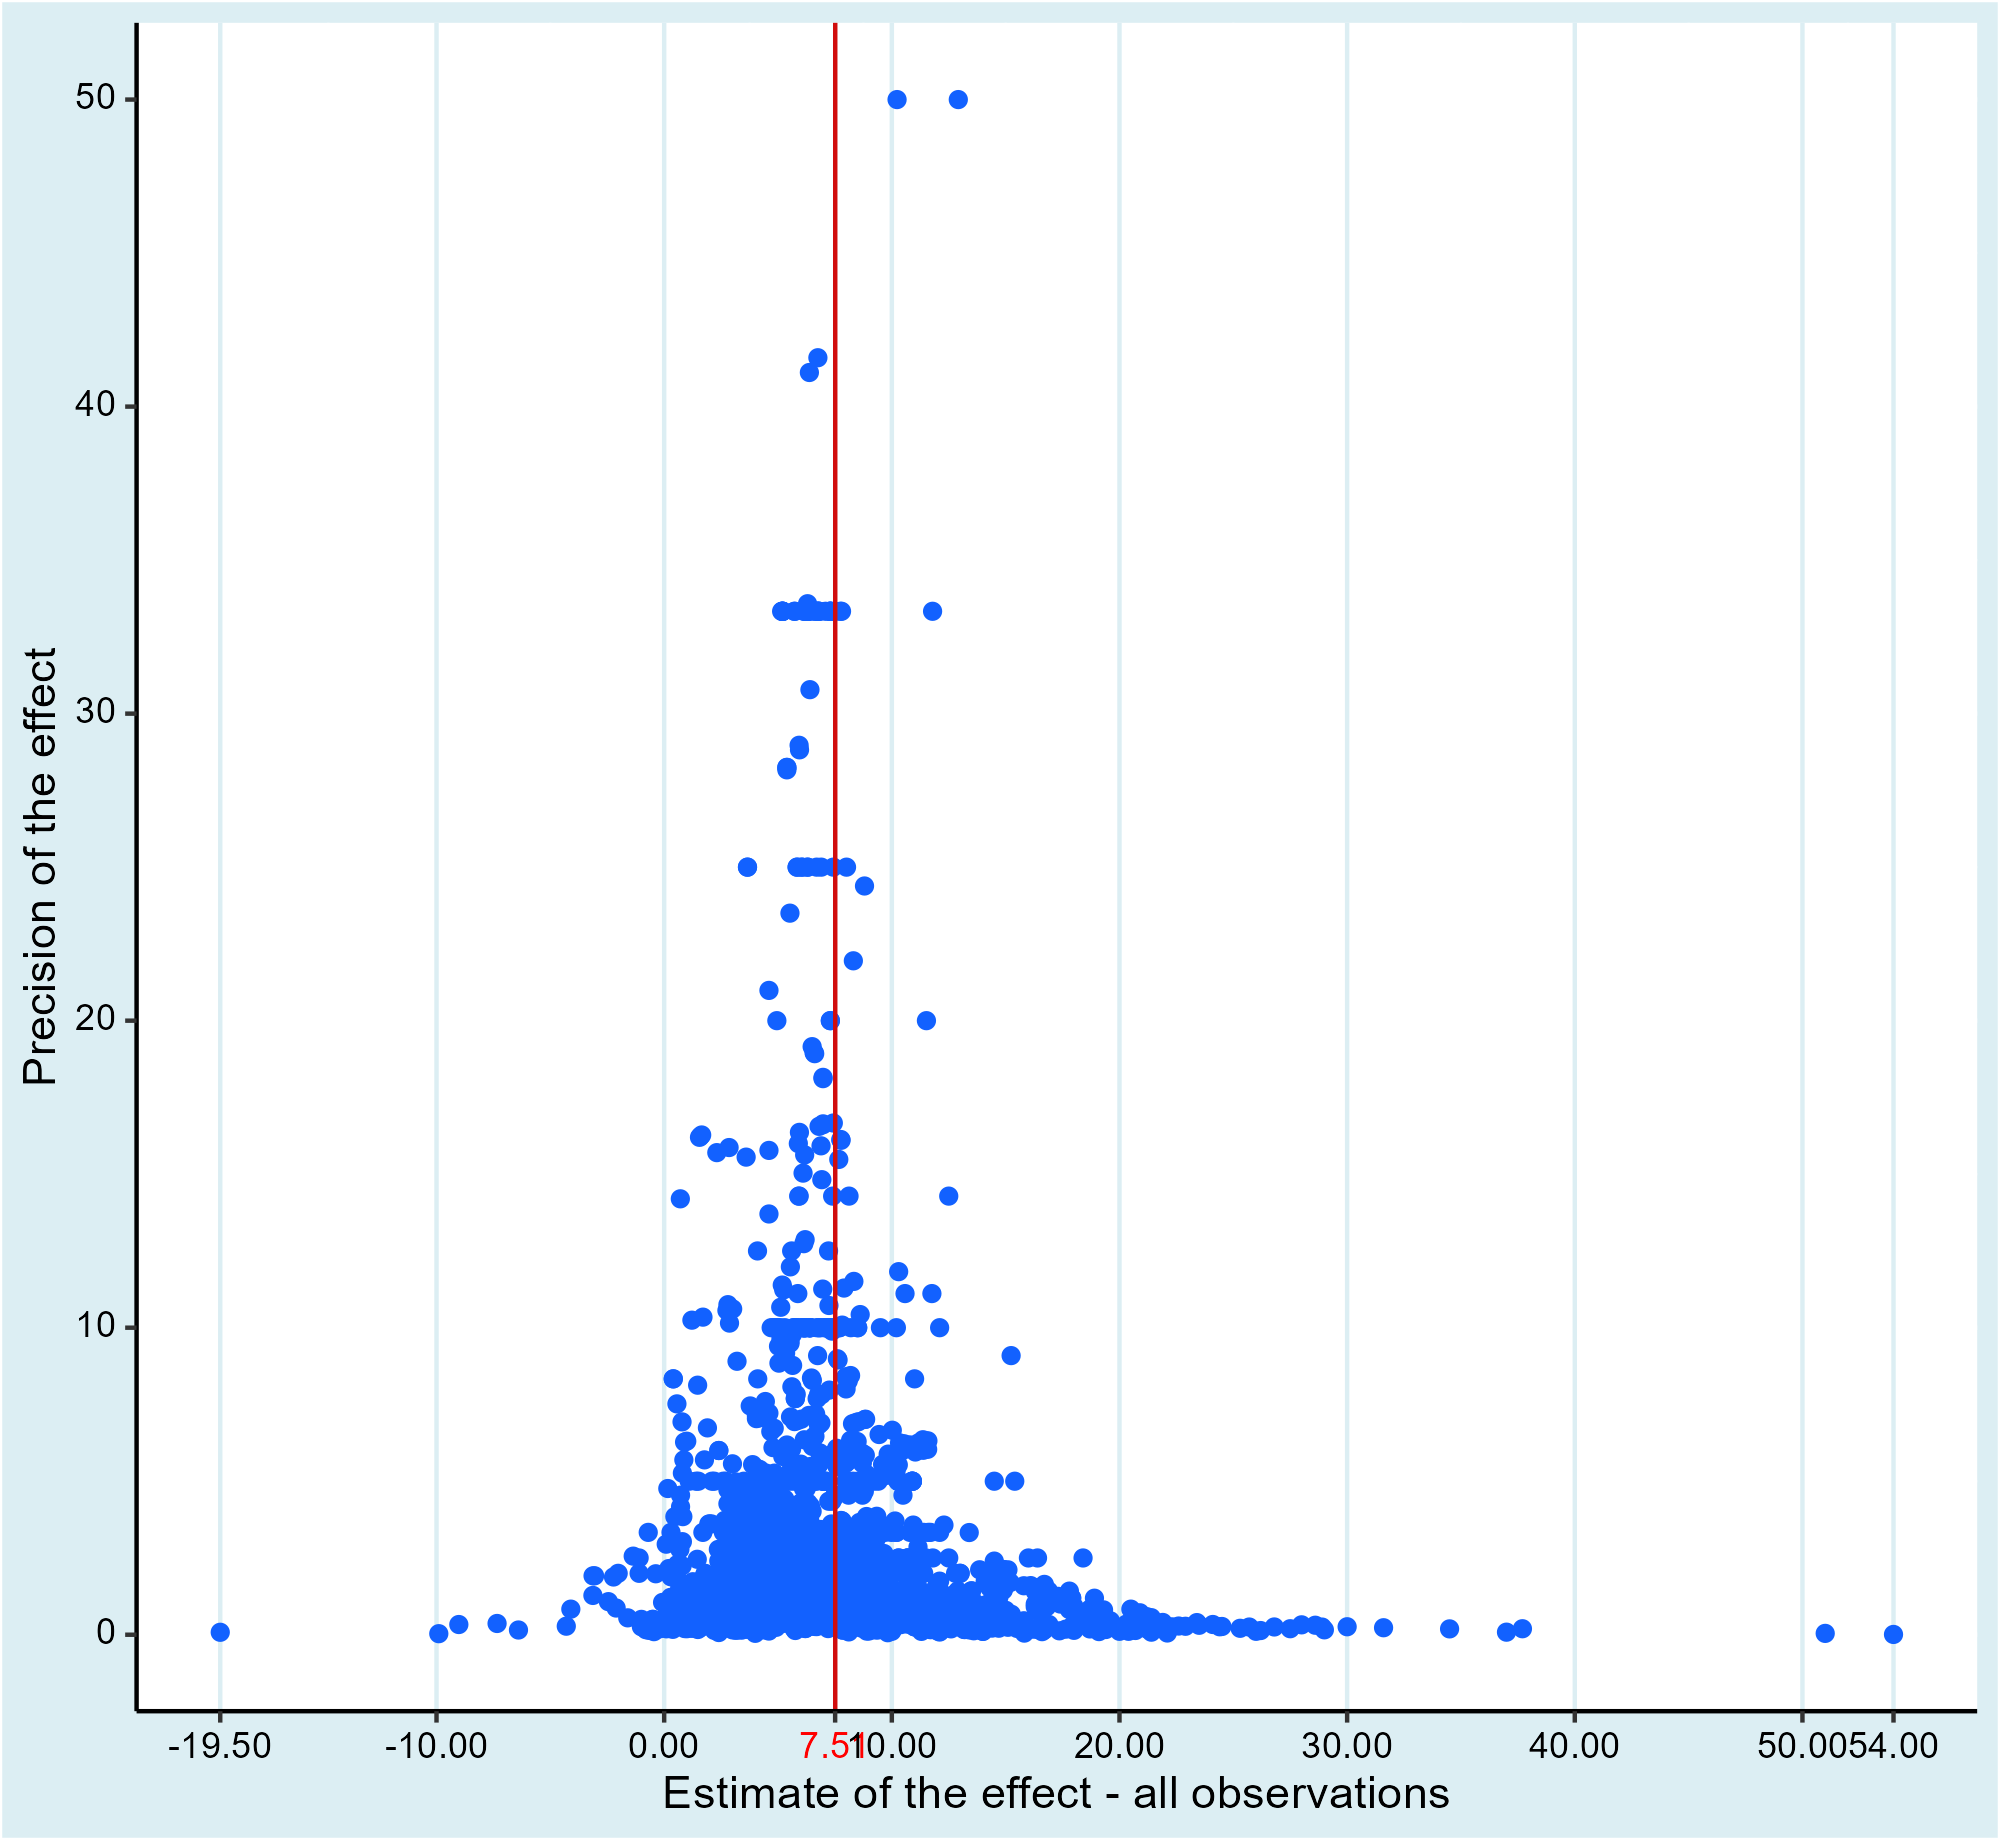
\includegraphics[width=0.65\textwidth]{Figures/funnel.png}
        \end{center}
    \end{figure}
\end{frame}



\begin{frame}{Statistical Tests and Publication Bias}
    \begin{tiny}

        \begin{table}[!t]
            \centering
            \begin{tabular}{
                @{}l*{6}{c}
                } %one left column, five center (*{} makes the cols inherit attributes)
                \toprule
                \multicolumn{1}{l}{}                  &
                \multicolumn{1}{c}{\textbf{OLS}}      &
                \multicolumn{1}{c}{\textbf{FE}}       &
                \multicolumn{1}{c}{\textbf{BE}}       &
                \multicolumn{1}{c}{\textbf{RE}}       &
                \multicolumn{1}{c}{\textbf{Study}}    &
                \multicolumn{1}{c}{\textbf{Precision}}                                                              \\
                \midrule
                Publication bias                      & 0.832   & 0.746   & 0.752   & 0.747   & 1.169     & 0.262   \\
                \emph{\hspace{0.2cm}(Standard error)} & (0.097) & (0.060) & (0.244) & (0.058) & (0.121)   & (0.425) \\
                \addlinespace[0.5em]
                Effect beyond bias                    & 6.408   & 6.517   & 6.741   & 6.708   & 6.294     & 6.540   \\
                \emph{\hspace{0.2cm}(Constant)}       & (0.118) & (0.107) & (0.418) & (0.294) & (0.153)   & (0.168) \\
                \addlinespace[0.5em]
                \toprule
                \addlinespace[0.5em]
                \multicolumn{1}{c}{}                  &
                \multicolumn{1}{c}{\textbf{WAAP}}     &
                \multicolumn{1}{c}{\textbf{Top10}}    &
                \multicolumn{1}{c}{\textbf{Stem}}     &
                \multicolumn{1}{c}{\textbf{Hier}}     &
                \multicolumn{1}{c}{\textbf{AK}}       &
                \multicolumn{1}{c}{\textbf{Kink}}                                                                   \\
                \midrule
                Publication bias                      &         &         &         & 0.503   & P = 2.764 & 0.262   \\
                                                      &         &         &         & (0.168) & (0.107)   & (0.39)  \\
                \addlinespace[0.5em]
                Effect beyond bias                    & 6.9     & 6.439   & 7.2     & 6.801   & 6.548     & 6.54    \\
                                                      & (0.092) & (0.548) & (1.186) & (0.266) & (0.091)   & (0.054) \\
                \addlinespace[0.5em]
                \midrule
                Observations                          & 1,754   & 1,754   & 1,754   & 1,754   & 1,754     & 1,754   \\

                \bottomrule
            \end{tabular}
        \end{table}

    \end{tiny}
\end{frame}



% \begin{frame}{Results Using Some Recent Methods}
%   \begin{tiny}

%     \begin{table}[!b]
%       \centering
%       \singlespace
%       \begin{tabular}{
%           l
%             *{4}{c}
%         }
%         \toprule

%         \multicolumn{5}{l}{\textit{Panel A: p-hacking tests by Elliott et al. (2022)}}                        \\
%         \addlinespace[0.3em]
%                                                         &
%         \textbf{Non-increas.}                           & \textbf{Monotonicity} &         &                   \\
%         \midrule
%         Non-increas.                                    & 0.819                 & 0.871   &         &         \\
%         Observations (p$\leq$0.1)                       & 1,610                 & 1,610   &         &         \\
%         Observations                                    & 1,754                 & 1,754   &         &         \\
%         \addlinespace[0.1em]
%         \hline

%         \addlinespace[0.5em]
%         \multicolumn{5}{l}{\textit{Panel B: MAIVE estimator (Irsova et al., 2023)}}                           \\
%         \addlinespace[0.3em]
%                                                         & \textbf{Results}      &         &         &         \\

%         \midrule
%         MAIVE coefficient                               & 5.736                 &         &         &         \\
%         Standard Error                                  & (0.460)               &         &         &         \\
%         F-test                                          & 12.491                &         &         &         \\
%         Observations                                    & 1,754                 &         &         &         \\
%         \addlinespace[0.1em]
%         \hline

%         \addlinespace[0.5em]
%         \multicolumn{5}{l}{\textit{Panel C: Robust Bayesian Model Averaging (Bartos et al., 2022)}}           \\
%         \addlinespace[0.3em]
%                                                         &
%         \multicolumn{1}{c}{\centering{\textbf{Mean}}}   &
%         \multicolumn{1}{c}{\centering{\textbf{Median}}} &
%         \multicolumn{1}{c}{\centering{\textbf{0.025}}}  &
%         \multicolumn{1}{c}{\centering{\textbf{0.975}}}                                                        \\
%         \midrule
%         Coefficient                                     & 7.125                 & 7.124   & 6.946   & 7.299   \\
%         Standard Error                                  & (3.505)               & (3.504) & (3.371) & (3.645) \\
%         Observations                                    & 1,754                 & 1,754   & 1,754   & 1,754   \\
%         \addlinespace[0.1em]
%         \bottomrule
%       \end{tabular}
%     \end{table}

%   \end{tiny}
% \end{frame}


\subsection{}

\begin{frame}{Individual Variables in Returns to Education}



    \begin{block}{Six categories of variables:}
        \begin{itemize}
            \item Estimates and their descriptive statistics
            \item Estimate characteristics
            \item Data characteristics
            \item Spatial/structural variation
            \item Estimation method
            \item Publication characteristics
        \end{itemize}
    \end{block}

\end{frame}

\begin{frame}{Different Approach to Ability}

    \begin{block}{Four ways to address ability:}
        \begin{itemize}
            \item Directly
            \item Indirectly
            \item Verbally
            \item Not at all
        \end{itemize}
    \end{block}


\end{frame}

\begin{frame}{Model Inclusion in Bayesian Model Averaging}
    \begin{center}
        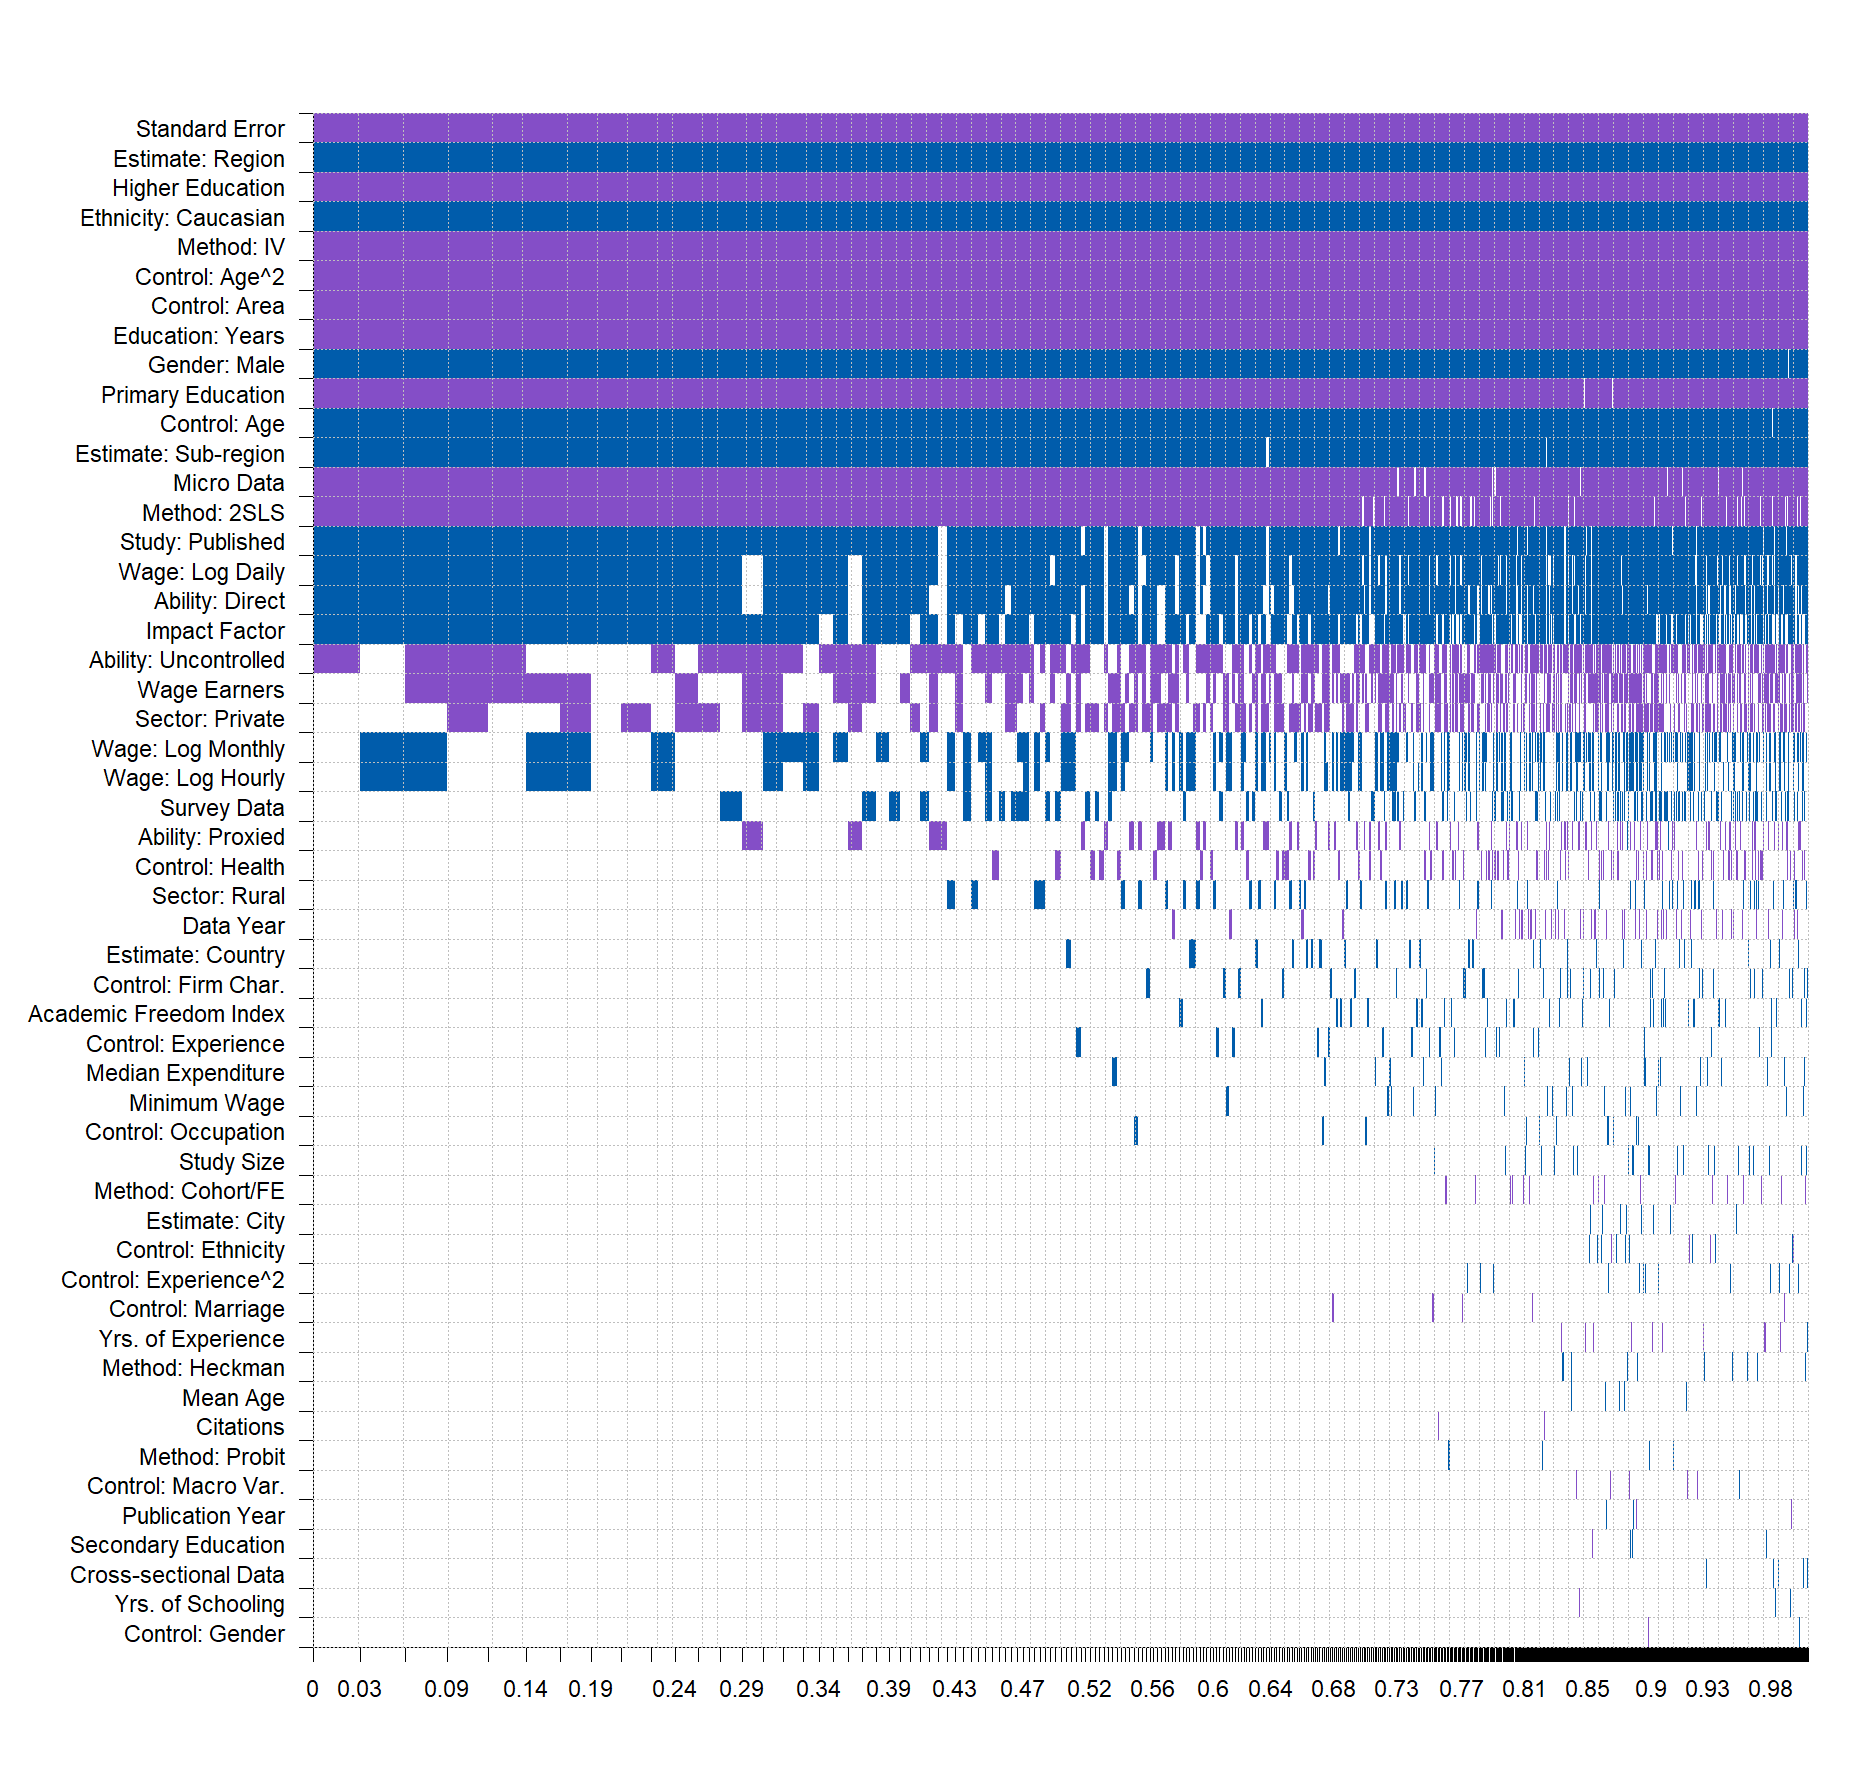
\includegraphics[width=0.7\textwidth]{Figures/bma_UIP_dilut_results.png}
    \end{center}
\end{frame}


% \begin{frame}{Economic Significance of Key Variables}


%   \newcommand{\colorcircle}[1]{
%     \begin{tikzpicture}
%       \pgfmathparse{ifthenelse(#1<0,"red","green")}
%       \fill[\pgfmathresult] (0,0) circle (0.8mm);
%     \end{tikzpicture}
%   }

%   \begin{tiny}
%     \begin{table}[!htbp]
%       \centering
%       \singlespace
%       \begin{tabular}{
%           @{}
%           l
%           *{4}{c}
%           @{}}
%         \toprule
%                                                   & \multicolumn{2}{c}{One SD change} & \multicolumn{2}{c}{Maximum change}                                \\
%                                                   & Effect on Returns                 & \% of BP                           & Effect on Returns & \% of BP \\
%         \midrule
%         \colorcircle{0.642} Standard Error        & 0.642                             & 9.82\%                             & 3.435             & 52.56\%  \\
%         \colorcircle{-0.428} Estimate: Sub-region & -0.428                            & -6.55\%                            & -1.433            & -21.92\% \\
%         \colorcircle{-0.612} Estimate: Region     & -0.612                            & -9.37\%                            & -1.325            & -20.27\% \\
%         \colorcircle{0.56} Education: Years       & 0.566                             & 8.67\%                             & 1.175             & 17.98\%  \\
%         \colorcircle{-0.40} Wage: Log Daily       & -0.405                            & -6.2\%                             & -1.384            & -21.18\% \\
%         \colorcircle{0.53} Micro Data             & 0.532                             & 8.13\%                             & 1.391             & 21.29\%  \\
%         \colorcircle{0.53} Primary Education      & 0.535                             & 8.18\%                             & 3.540             & 54.16\%  \\
%         \colorcircle{1.366} Higher Education      & 1.366                             & 20.91\%                            & 5.521             & 84.48\%  \\
%         \colorcircle{-0.42} Gender: Male          & -0.425                            & -6.5\%                             & -1.215            & -18.58\% \\
%         \colorcircle{-0.60} Ethnicity: Caucasian  & -0.608                            & -9.3\%                             & -1.449            & -22.18\% \\
%         \colorcircle{0.43} Method: 2SLS           & 0.433                             & 6.62\%                             & 1.474             & 22.56\%  \\
%         \colorcircle{0.824} Method: IV            & 0.824                             & 12.61\%                            & 2.627             & 40.2\%   \\
%         \colorcircle{-0.388} Ability: Direct      & -0.388                            & -5.94\%                            & -1.138            & -17.41\% \\
%         \colorcircle{0.27} Ability: Uncontrolled  & 0.271                             & 4.15\%                             & 0.548             & 8.39\%   \\
%         \colorcircle{-0.89} Control: Age          & -0.895                            & -13.69\%                           & -1.883            & -28.81\% \\
%         \colorcircle{1.315} Control: Age$^2$      & 1.315                             & 20.12\%                            & 2.945             & 45.06\%  \\
%         \colorcircle{0.878} Control: Area         & 0.878                             & 13.44\%                            & 1.781             & 27.24\%  \\
%         \colorcircle{-0.296} Impact Factor        & -0.296                            & -4.53\%                            & -1.349            & -20.64\% \\
%         \colorcircle{-0.44} Study: Published      & -0.445                            & -6.8\%                             & -1.047            & -16.01\% \\
%         \bottomrule
%       \end{tabular}
%     \end{table}
%   \end{tiny}
% \end{frame}


% %\begin{frame}{Best-Practice Estimate Across Literature}
% %
% %\begin{table}[!htbp]
% %\centering
% %\scriptsize
% %\singlespace
% %\begin{tabular}{
% %@{}
% %l
% %*{3}{c}
% %@{}}
% %\toprule
% %    \textbf{Study} & \textbf{Estimate} & \textbf{95\% Confidence Interval} & \textbf{Studies} \\
% %\midrule
% %    Author & 6.536 & (5.762; 7.310)  & 0\\
% %    Query & 7.529 & (3.552; 11.506) & 74\\
% %    Snowballing & 6.346 & (2.530; 10.162) & 41\\
% %    All studies & 7.109 & (3.046; 11.17) & 115\\
% %\bottomrule
% %\end{tabular}
% %\end{table}
% %
% %\end{frame}

% \begin{frame}{Ability Matters}
%   \begin{center}
%     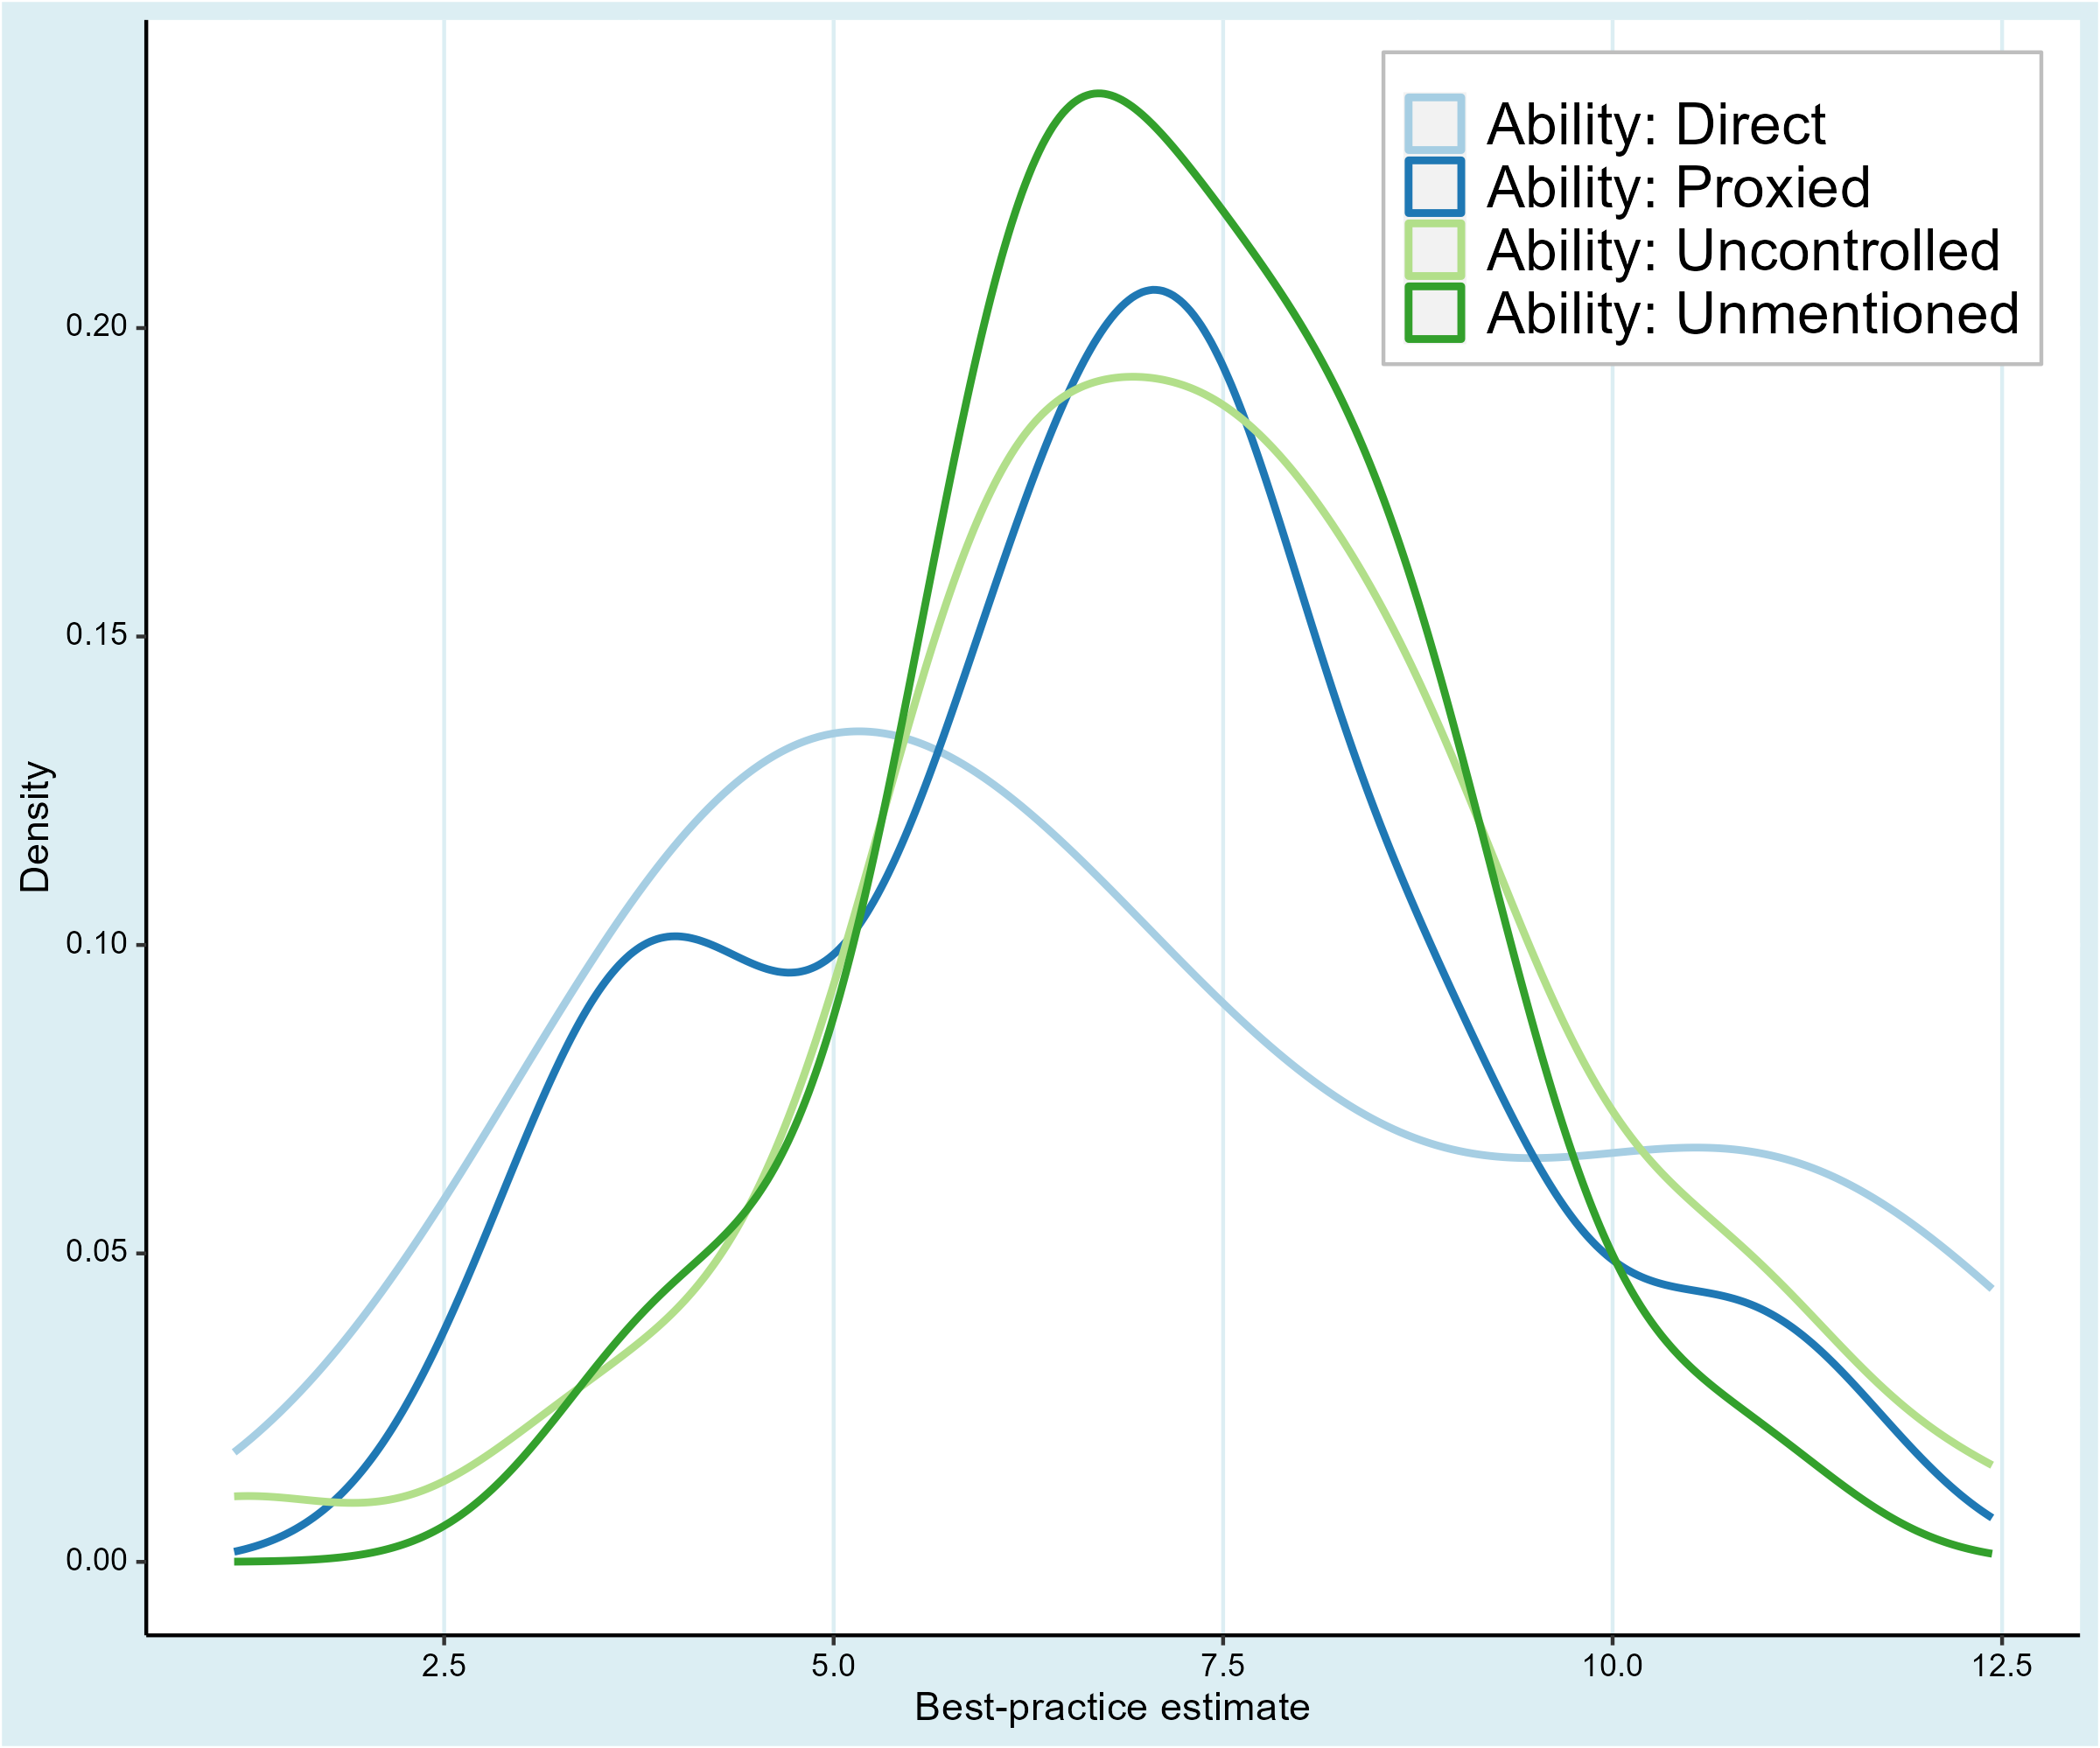
\includegraphics[width=0.7\textwidth]{Figures/bpe_ability.png}
%   \end{center}
% \end{frame}



% \begin{frame}{What we learned}
%   \begin{block}{Main Findings}
%     \begin{enumerate}
%       \item
%             An overall effect of returns to schooling drops roughly one percentage point (7\% to 6\%) after corrected for publication bias
%       \item
%             Ability matters, and controlling for it in the regression decreases the expected returns to schooling
%       \item
%             Nine variables have a significant positive influence on returns to schooling, while ten have a negative one
%     \end{enumerate}
%   \end{block}


% \end{frame}

% \section{Extensions}
% \subsection{}

% \begin{frame}{There's more...}

%   \begin{center}
%     \begin{LARGE}
%       Technology
%     \end{LARGE}
%   \end{center}

% \end{frame}

% \begin{frame}{Stages of Meta-Analysis}
%   \centering
%   \Large
%   \begin{tikzpicture}[node distance=1.3cm]
%     \node (idea) {Idea};
%     \node (data) [below of=idea] {Data};
%     \node (analysis) [below of=data] {Analysis};
%     \node (writing) [below of=analysis] {Writing};
%     \node (results) [below of=writing] {Results};

%     \draw[->] (idea) -- (data);
%     \draw[->] (data) -- (analysis);
%     \draw[->] (analysis) -- (writing);
%     \draw[->] (writing) -- (results);

%     \only<2>{\draw[red,thick] (analysis.south west) -- (analysis.north east);}
%   \end{tikzpicture}
% \end{frame}



% \begin{frame}{Let's get technical}

%   \begin{itemize}
%     \item Meta-analysis, but automatized
%     \item One script and a bit of parametrization
%     \item Faster methods, all ran locally
%     \item Caches and file handling
%     \item All results calculated, formatted, and exported within minutes
%   \end{itemize}

% \end{frame}


% \begin{frame}[fragile]{Project structure}

%   \begin{scriptsize}
%     \begin{forest}
%       for tree={
%       grow'=0,
%       child anchor=west,
%       parent anchor=south,
%       anchor=west,
%       calign=first,
%       edge path={
%           \noexpand\path [draw, \forestoption{edge}]
%           (!u.south west) +(7.5pt,0) |- (.child anchor) pic {folder} \forestoption{edge label};
%         },
%       font=\ttfamily,
%       before typesetting nodes={
%           if n=1
%             {insert before={[,phantom]}}
%             {}
%         },
%       fit=band,
%       before computing xy={l=15pt},
%       }
%       [.
%       [data/ ]
%       [pckg/ ]
%       [scripts/ ]
%       [results/
%       [graphic/]
%       [numeric/]
%       [main\_results.txt]
%       ]
%       [main\_master\_thesis\_cala.R]
%       [script\_runner\_master\_thesis\_cala.R]
%       [source\_master\_thesis\_cala.R]
%       [README.md]
%       [user\_parameters.yaml]
%       ]
%     \end{forest}
%   \end{scriptsize}

% \end{frame}

% \begin{frame}{Graphic Results}
%   \begin{center}
%     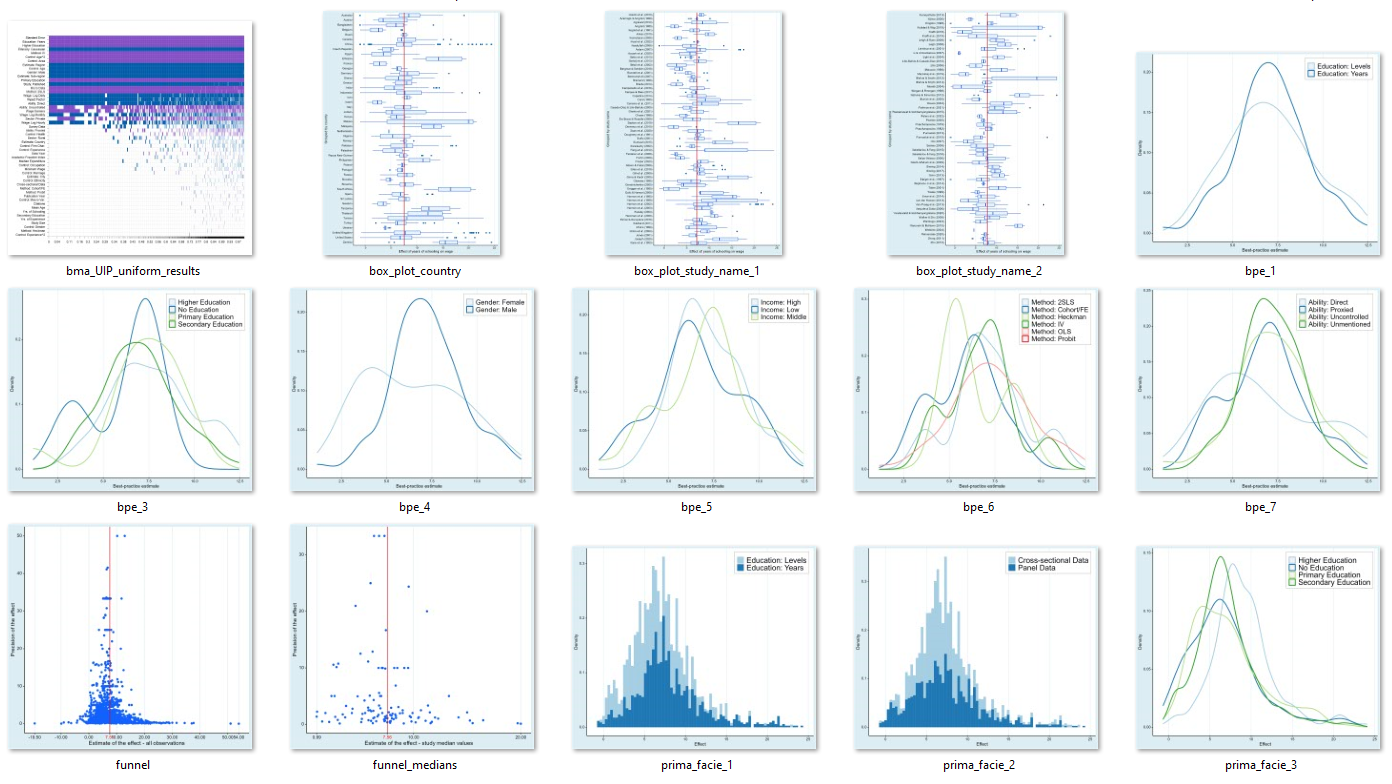
\includegraphics[width=1\textwidth]{Figures/graphical_results.png}
%   \end{center}
% \end{frame}


% \begin{frame}{Numeric Results}
%   \begin{center}
%     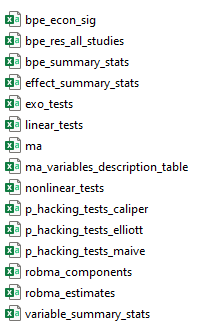
\includegraphics[width=0.4\textwidth]{Figures/numeric_results.png}
%   \end{center}
% \end{frame}

% \begin{frame}{main\_results.txt}
%   \begin{center}
%     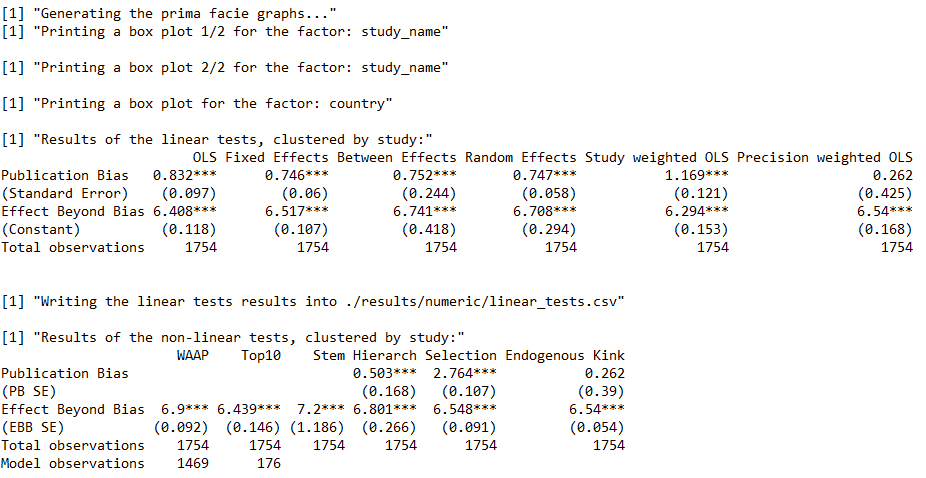
\includegraphics[width=1\textwidth]{Figures/main_results.png}
%   \end{center}
% \end{frame}


% \begin{frame}{It can do this...}
%   \begin{itemize}
%     \item Variable summary statistics
%     \item Effect summary statistics
%     \item Prima Facie graphs
%     \item Box plot
%     \item Funnel plot
%     \item T-statistic histogram
%     \item Linear tests
%           \begin{itemize}
%             \item OLS
%             \item Between Effects
%             \item Fixed Effects
%             \item Random Effects
%             \item Study-weighted OLS
%             \item Precision-weighted OLS
%           \end{itemize}
%   \end{itemize}
% \end{frame}



% \begin{frame}{...and this...}
%   \begin{itemize}

%     \item Non-linear tests
%           \begin{itemize}
%             \item Weighted Average of Adequately Powered
%             \item Top10
%             \item Stem-based method
%             \item Hierarchial Bayes
%             \item Selection model
%             \item Endogenous Kink model
%           \end{itemize}
%     \item Tests relaxing exogeneity
%           \begin{itemize}
%             \item Instrumental Variable regression
%             \item p-uniform*
%           \end{itemize}
%     \item P-hacking tests
%           \begin{itemize}
%             \item Caliper tests
%             \item Elliott tests
%             \item MAIVE estimator
%           \end{itemize}

%   \end{itemize}
% \end{frame}

% \begin{frame}{...and even this!}
%   \begin{itemize}


%     \item Bayesian Model Averaging
%     \item Frequentist Model Averaging
%     \item Model Averaging variables description table
%     \item Best-practice estimate
%     \item Best-practice estimate: Graphs
%     \item Best-practice estimate: Summary statistics
%     \item Robust Bayesian Model Averaging
%   \end{itemize}
% \end{frame}


% \begin{frame}{Available on GitHub}

%   \begin{center}
%     
\includegraphics[width=0.08\textwidth]{Figures/github.png}

%     \vspace{0.5cm}

%     \begin{Large}
%       github.com/PetrCala/Diploma-Thesis \\
%     \end{Large}

%   \end{center}

% \end{frame}




% % All of the following is optional and typically not needed. 
% %\appendix
% %\section<presentation>*{\appendixname}
% %\subsection<presentation>*{For Further Reading}




% \appendix



% \begin{frame}
%   \frametitle<presentation>{}

%   \begin{center}
%     \begin{LARGE}
%       Thank you!
%     \end{LARGE}
%   \end{center}

% \end{frame}

% \begin{frame}%[allowframebreaks]
%   \frametitle<presentation>{References}

%   \begin{thebibliography}{10}

%     %\beamertemplatebookbibitems
%     % Start with overview books.


%     \beamertemplatearticlebibitems
%     % Followed by interesting articles. Keep the list short. 

%     \bibitem[{Becker(1962)}]{Becker1962}
%     Becker, Gary S. "Investment in human capital: A theoretical analysis."
%     \newblock\emph{Journal of political economy} 70, no. 5, Part 2 (1962): 9-49.
%     \bibitem[{Mincer (1974)}]{Mincer1974}
%     Mincer, Jacob. "Schooling, Experience, and Earnings. Human Behavior & Social Institutions No. 2."
%     \bibitem[{Ree et al. (1994)}]{Ree1994}
%     Ree, Malcolm James, James A. Earles, and Mark S. Teachout. "Predicting job performance: Not much more than g.."
%     \newblock\emph{Journal of applied psychology 79, no. 4}: 518.
%     \bibitem[{Griliches (1977)}]{Griliches1977}
%     Griliches, Zvi. "Estimating the returns to schooling: Some econometric problems."
%     \newblock\emph{Journal of political economy}: 1-22.
%   \end{thebibliography}
% \end{frame}


% \begin{frame}{Making a twin dataset}

%   \begin{itemize}
%     \item What if we could observe subjects with identical inherent ability?
%     \item Make a dataset comprised of twin subjects!
%     \item 16 twin studies with 293 observations
%     \item Differences in methodology $\to$ ability bias
%   \end{itemize}

% \end{frame}

% \begin{frame}{Are the results just identical?}

%   \begin{tiny}
%     \begin{table}[!t]
%       \centering
%       \singlespace
%       \begin{tabular}{
%           @{}
%           l % Description
%           *{7}{c} % Middle columns
%           %>{\centering\arraybackslash}p{1cm} % Last column with fixed width
%           @{}
%         }
%         \toprule
%                                      & \multicolumn{3}{c}{Unweighted} & \multicolumn{3}{c}{Weighted}        &                                                                      \\
%         \cmidrule(lr){2-4} \cmidrule(lr){5-7}
%                                      & Mean                           & \multicolumn{2}{c}{95\% conf. int.} & Mean   & \multicolumn{2}{c}{95\% conf. int.} & N. obs                \\

%         \midrule


%         \multicolumn{8}{l}{\textit{Baseline methods}}                                                                                                                              \\
%         Method: OLS                  & 5.686                          & 1.648                               & 9.724  & 5.754                               & 1.716  & 9.792  & 101 \\
%         Method: GLS                  & 7.363                          & 1.822                               & 12.904 & 8.005                               & 2.464  & 13.546 & 30  \\
%         Method: IV                   & 7.155                          & 1.644                               & 12.666 & 7.570                               & 2.059  & 13.081 & 58  \\
%         \midrule
%         \multicolumn{8}{l}{\textit{Methods that treat the omitted ability bias}}                                                                                                   \\
%         Method: Selection/FE         & 4.917                          & 0.515                               & 9.319  & 5.630                               & 1.228  & 10.032 & 74  \\
%         Method: First Differences    & 7.920                          & 3.979                               & 11.861 & 7.916                               & 3.975  & 11.857 & 10  \\
%         Method: IV First-Differenced & 8.689                          & 1.035                               & 16.343 & 8.725                               & 1.071  & 16.379 & 20  \\

%         \bottomrule
%       \end{tabular}
%     \end{table}

%   \end{tiny}
% \end{frame}

% \begin{frame}{Graphing out the individual method differences}
%   \begin{center}
%     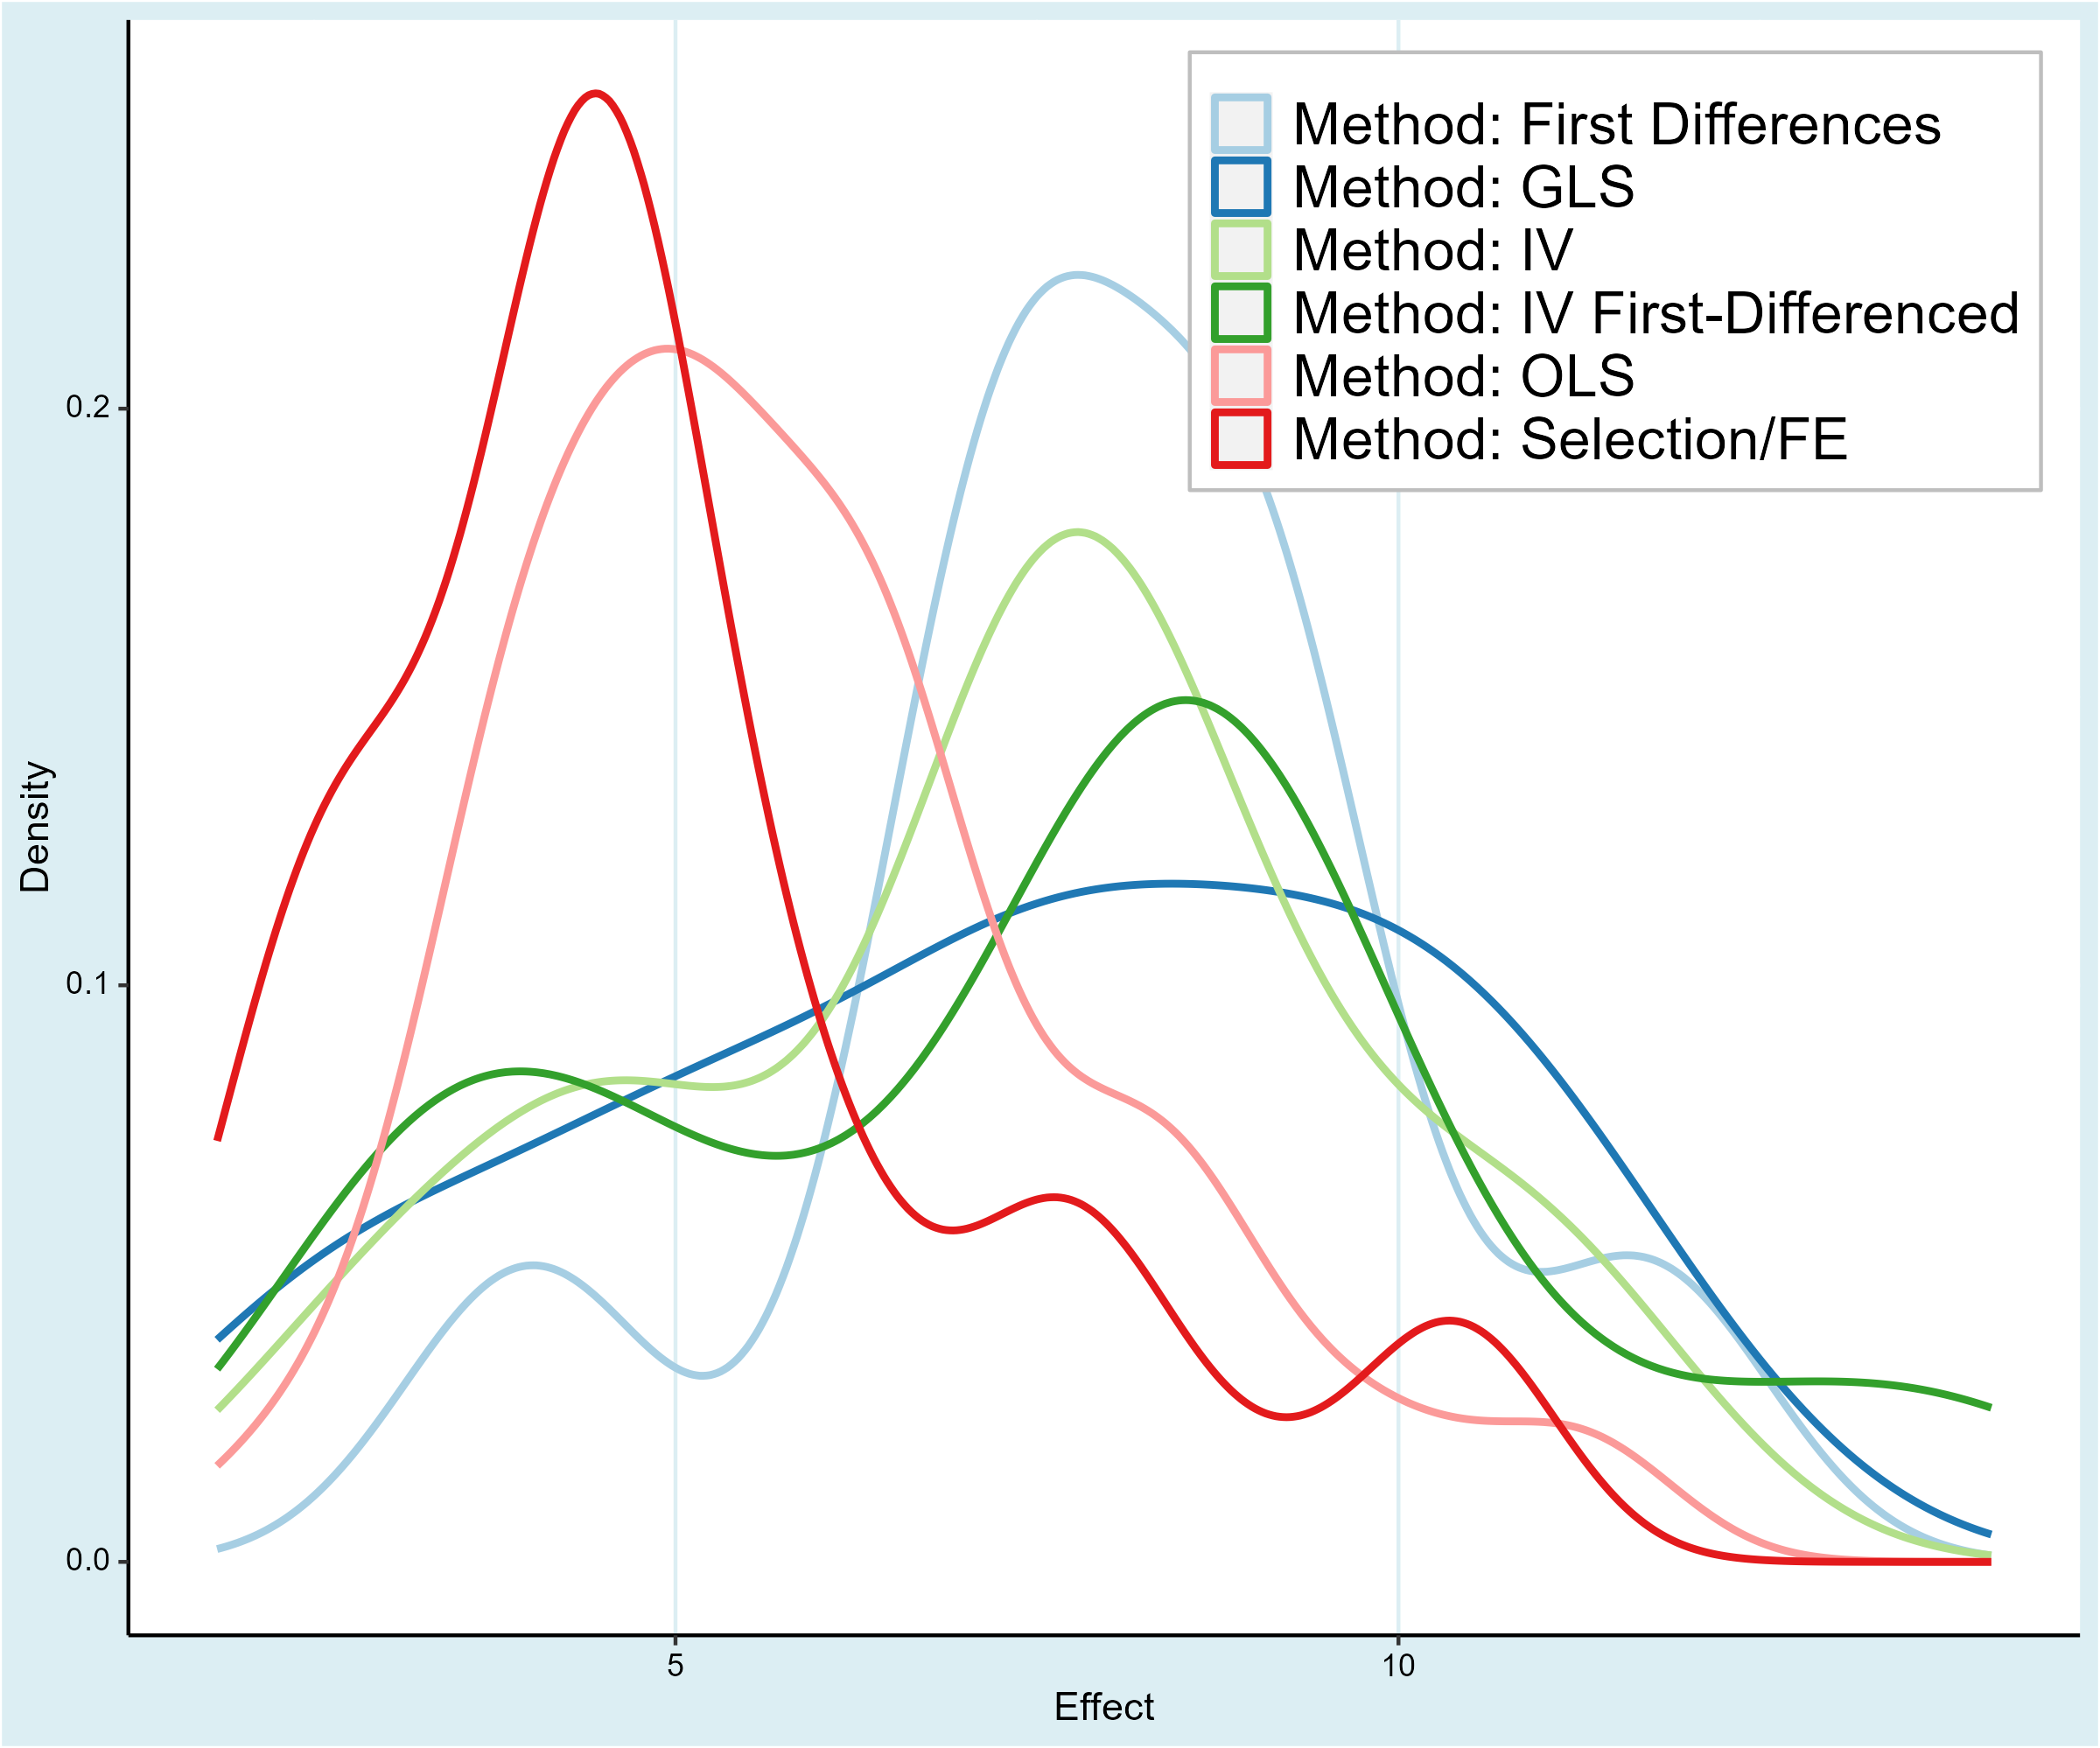
\includegraphics[width=0.7\textwidth]{Figures/twins_prima_method.png}
%   \end{center}
% \end{frame}



% \begin{frame}{Publication bias revisited}
%   \begin{tiny}
%     \begin{table}[!htbp]
%       \centering
%       \singlespace
%       \begin{tabular}{
%           @{\hskip\tabcolsep\extracolsep}
%           l*{6}{c}} %one left column, five center (*{} makes the cols inherit attributes)
%         \toprule
%         \multicolumn{1}{c}{}                  &
%         \textbf{OLS}                          &
%         \textbf{FE}                           &
%         \textbf{BE}                           &
%         \textbf{RE}                           &
%         \textbf{Study}                        &
%         \textbf{Precision}                                                                                \\
%         \midrule

%         Publication bias                      & 1.347   & 0.602   & 2.133   & 0.840   & 0.947   & 2.897   \\
%         \emph{\hspace{0.2cm}(Standard error)} & (0.138) & (0.162) & (0.505) & (0.154) & (0.177) & (0.442) \\
%         \addlinespace[0.5em]
%         Effect beyond bias                    & 4.735   & 5.574   & 4.106   & 5.55    & 4.754   & 3.907   \\
%         \emph{\hspace{0.2cm}(Constant)}       & (0.175) & (0.219) & (0.711) & (0.342) & (0.185) & (0.232) \\

%         \midrule

%                                               &
%         \textbf{WAAP}                         &
%         \textbf{Top10}                        &
%         \textbf{Stem}                         &
%         \textbf{Hier}                         &
%         \textbf{AK}                           &
%         \textbf{Kink}                                                                                     \\
%         \midrule
%         Publication bias                      &         &         &         & 0.601   & 2.257   & 2.895   \\
%                                               &         &         &         & (0.365) & (0.126) & (0.435) \\
%         \addlinespace[0.5em]
%         Effect beyond bias                    & 5.77    & 4.314   & 3.403   & 5.857   & 5.616   & 3.908   \\
%                                               & (0.159) & (0.265) & (0.95)  & (0.544) & (0.157) & (0.093) \\

%         \midrule
%         \addlinespace[0.5em]
%         Observations                          & 293     & 293     & 293     & 293     & 293     & 293     \\

%         \bottomrule
%       \end{tabular}
%     \end{table}

%   \end{tiny}
% \end{frame}


\end{document}


